\documentclass{standalone}
\usepackage{tikz}
\usetikzlibrary{patterns, positioning}
\usepackage[sfdefault]{ClearSans} %% option 'sfdefault' activates Clear Sans as the default text font
\usepackage[T1]{fontenc}

\begin{document}
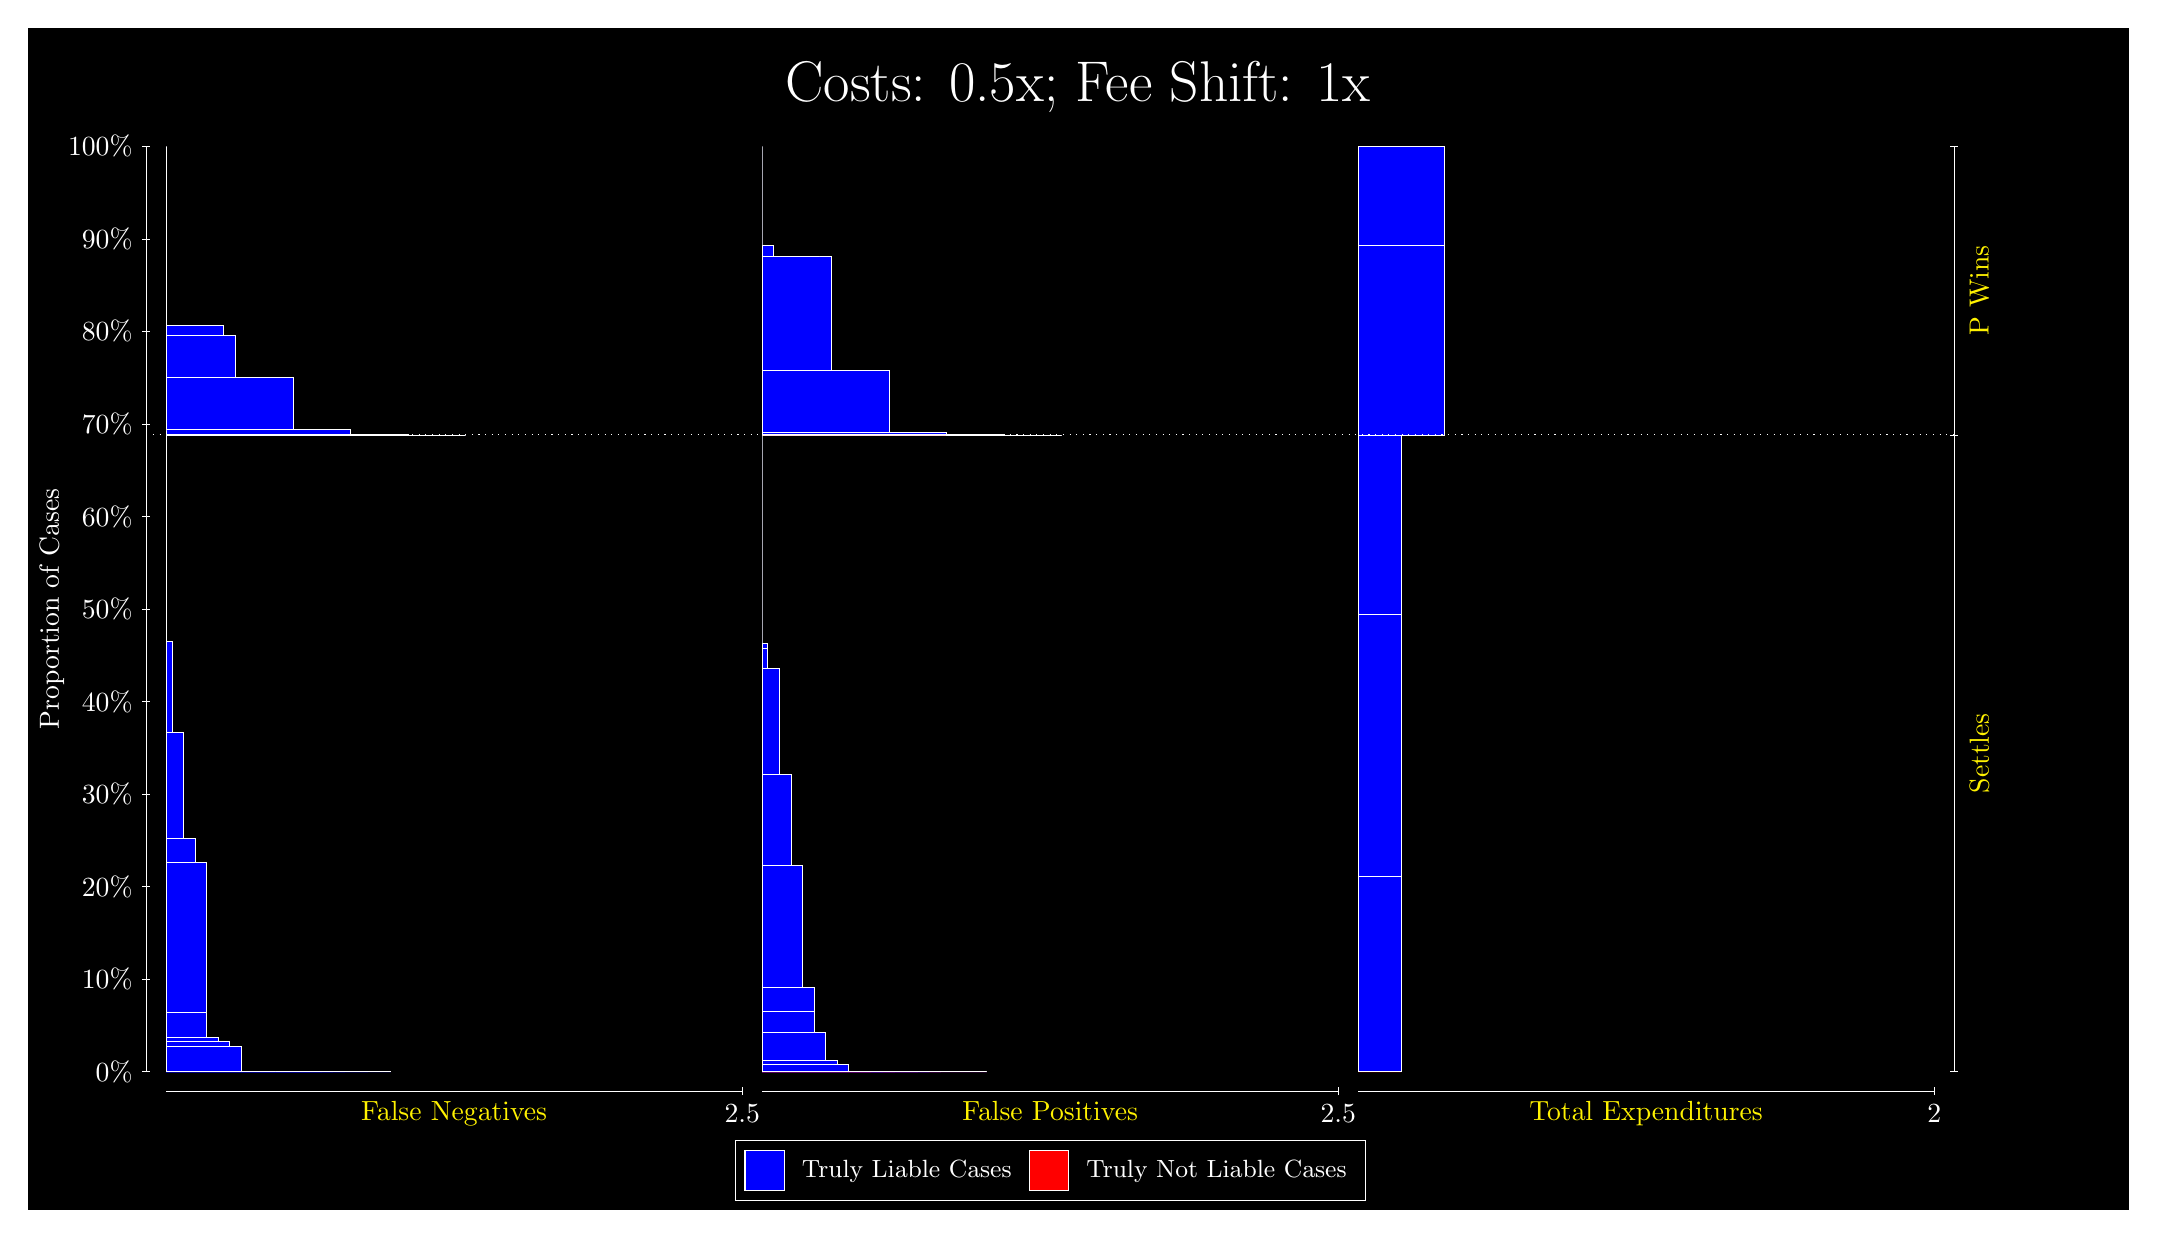
\begin{tikzpicture}
\draw[fill=black] (0,0) rectangle (26.667,15);
\draw[text=white] (0,13.5) rectangle (26.667,15) node[midway] {\huge Costs: 0.5x; Fee Shift: 1x};
\draw[white, very thin] (1.5,1.75) -- (1.5,13.5);
\node[rotate=90, text=white, anchor=center] at (0.3, 7.625) {Proportion of Cases};
\draw[white, very thin] (1.45,1.75) -- (1.55,1.75);
\node[text=white, anchor=east] at (1.45, 1.75) {0\%};
\draw[white, very thin] (1.45,2.925) -- (1.55,2.925);
\node[text=white, anchor=east] at (1.45, 2.925) {10\%};
\draw[white, very thin] (1.45,4.1) -- (1.55,4.1);
\node[text=white, anchor=east] at (1.45, 4.1) {20\%};
\draw[white, very thin] (1.45,5.275) -- (1.55,5.275);
\node[text=white, anchor=east] at (1.45, 5.275) {30\%};
\draw[white, very thin] (1.45,6.45) -- (1.55,6.45);
\node[text=white, anchor=east] at (1.45, 6.45) {40\%};
\draw[white, very thin] (1.45,7.625) -- (1.55,7.625);
\node[text=white, anchor=east] at (1.45, 7.625) {50\%};
\draw[white, very thin] (1.45,8.8) -- (1.55,8.8);
\node[text=white, anchor=east] at (1.45, 8.8) {60\%};
\draw[white, very thin] (1.45,9.975) -- (1.55,9.975);
\node[text=white, anchor=east] at (1.45, 9.975) {70\%};
\draw[white, very thin] (1.45,11.15) -- (1.55,11.15);
\node[text=white, anchor=east] at (1.45, 11.15) {80\%};
\draw[white, very thin] (1.45,12.325) -- (1.55,12.325);
\node[text=white, anchor=east] at (1.45, 12.325) {90\%};
\draw[white, very thin] (1.45,13.5) -- (1.55,13.5);
\node[text=white, anchor=east] at (1.45, 13.5) {100\%};

\draw[white, very thin] (24.457,1.75) -- (24.457,13.5);
\draw[white, very thin] (24.407,1.75) -- (24.507,1.75);
\node[anchor=west] at (24.407, 1.75) {};
\draw[white, very thin] (24.407,9.8365) -- (24.507,9.8365);
\node[anchor=west] at (24.407, 9.8365) {};
\draw[white, very thin] (24.407,13.5) -- (24.507,13.5);
\node[anchor=west] at (24.407, 13.5) {};

\draw[white, very thin, fill=blue] (1.75,1.75) rectangle (4.6044,1.75);
\draw[white, very thin, fill=blue] (1.75,1.75) rectangle (4.3116,1.75);
\draw[white, very thin, fill=blue] (1.75,1.75) rectangle (4.0188,1.75);
\draw[white, very thin, fill=blue] (1.75,1.75) rectangle (3.8725,1.75);
\draw[white, very thin, fill=blue] (1.75,1.75) rectangle (3.7261,1.75);
\draw[white, very thin, fill=blue] (1.75,1.75) rectangle (3.5797,1.75);
\draw[white, very thin, fill=blue] (1.75,1.75) rectangle (3.4333,1.7507);
\draw[white, very thin, fill=blue] (1.75,1.7507) rectangle (3.287,1.7507);
\draw[white, very thin, fill=blue] (1.75,1.7507) rectangle (3.1406,1.7507);
\draw[white, very thin, fill=blue] (1.75,1.7507) rectangle (2.9942,1.7534);
\draw[white, very thin, fill=blue] (1.75,1.7534) rectangle (2.8478,1.757);
\draw[white, very thin, fill=blue] (1.75,1.757) rectangle (2.7015,2.0683);
\draw[white, very thin, fill=blue] (1.75,2.0683) rectangle (2.5551,2.1291);
\draw[white, very thin, fill=blue] (1.75,2.1291) rectangle (2.4087,2.1879);
\draw[white, very thin, fill=blue] (1.75,2.1879) rectangle (2.2623,2.4985);
\draw[white, very thin, fill=blue] (1.75,2.4985) rectangle (2.2623,4.4022);
\draw[white, very thin, fill=blue] (1.75,4.4022) rectangle (2.1159,4.7136);
\draw[white, very thin, fill=blue] (1.75,4.7136) rectangle (1.9696,6.0612);
\draw[white, very thin, fill=blue] (1.75,6.0612) rectangle (1.8232,7.2183);
\draw[white, very thin, fill=red] (1.75,7.2183) rectangle (1.75,7.2183);
\draw[white, very thin, fill=blue] (1.75,7.2183) rectangle (1.75,9.8365);
\draw[white, very thin, fill=blue] (1.75,9.8365) rectangle (5.5558,9.8365);
\draw[white, very thin, fill=blue] (1.75,9.8365) rectangle (4.8239,9.8375);
\draw[white, very thin, fill=blue] (1.75,9.8375) rectangle (4.092,9.9028);
\draw[white, very thin, fill=blue] (1.75,9.9028) rectangle (3.9457,9.9028);
\draw[white, very thin, fill=blue] (1.75,9.9028) rectangle (3.3602,10.571);
\draw[white, very thin, fill=blue] (1.75,10.571) rectangle (3.2138,10.571);
\draw[white, very thin, fill=blue] (1.75,10.571) rectangle (2.6283,11.094);
\draw[white, very thin, fill=blue] (1.75,11.094) rectangle (2.4819,11.231);
\draw[white, very thin, fill=blue] (1.75,11.231) rectangle (1.8964,11.232);
\draw[white, very thin, fill=red] (1.75,11.232) rectangle (1.75,11.232);
\draw[white, very thin, fill=blue] (1.75,11.232) rectangle (1.75,13.5);
\draw[white, very thin, fill=red] (9.3189,1.75) rectangle (12.173,1.75);
\draw[white, very thin, fill=blue] (9.3189,1.75) rectangle (12.173,1.75);
\draw[white, very thin, fill=red] (9.3189,1.75) rectangle (11.588,1.75);
\draw[white, very thin, fill=blue] (9.3189,1.75) rectangle (11.588,1.75);
\draw[white, very thin, fill=blue] (9.3189,1.75) rectangle (11.441,1.75);
\draw[white, very thin, fill=red] (9.3189,1.75) rectangle (11.295,1.75);
\draw[white, very thin, fill=blue] (9.3189,1.75) rectangle (11.295,1.75);
\draw[white, very thin, fill=red] (9.3189,1.75) rectangle (11.002,1.75);
\draw[white, very thin, fill=blue] (9.3189,1.75) rectangle (11.002,1.75);
\draw[white, very thin, fill=blue] (9.3189,1.75) rectangle (10.856,1.75);
\draw[white, very thin, fill=red] (9.3189,1.75) rectangle (10.709,1.75);
\draw[white, very thin, fill=blue] (9.3189,1.75) rectangle (10.709,1.7507);
\draw[white, very thin, fill=blue] (9.3189,1.7507) rectangle (10.709,1.7512);
\draw[white, very thin, fill=blue] (9.3189,1.7512) rectangle (10.563,1.7512);
\draw[white, very thin, fill=red] (9.3189,1.7512) rectangle (10.417,1.7512);
\draw[white, very thin, fill=blue] (9.3189,1.7512) rectangle (10.417,1.8364);
\draw[white, very thin, fill=blue] (9.3189,1.8364) rectangle (10.27,1.8952);
\draw[white, very thin, fill=red] (9.3189,1.8952) rectangle (10.124,1.8952);
\draw[white, very thin, fill=blue] (9.3189,1.8952) rectangle (10.124,2.2518);
\draw[white, very thin, fill=blue] (9.3189,2.2518) rectangle (10.124,2.2539);
\draw[white, very thin, fill=blue] (9.3189,2.2539) rectangle (9.9776,2.5091);
\draw[white, very thin, fill=blue] (9.3189,2.5091) rectangle (9.9776,2.8205);
\draw[white, very thin, fill=red] (9.3189,2.8205) rectangle (9.8312,2.8205);
\draw[white, very thin, fill=blue] (9.3189,2.8205) rectangle (9.8312,4.3678);
\draw[white, very thin, fill=blue] (9.3189,4.3678) rectangle (9.8312,4.3683);
\draw[white, very thin, fill=blue] (9.3189,4.3683) rectangle (9.6848,5.5253);
\draw[white, very thin, fill=blue] (9.3189,5.5253) rectangle (9.5384,6.873);
\draw[white, very thin, fill=blue] (9.3189,6.873) rectangle (9.3921,7.126);
\draw[white, very thin, fill=blue] (9.3189,7.126) rectangle (9.3921,7.1843);
\draw[white, very thin, fill=blue] (9.3189,7.1843) rectangle (9.3189,9.8365);
\draw[white, very thin, fill=red] (9.3189,9.8365) rectangle (13.125,9.8365);
\draw[white, very thin, fill=blue] (9.3189,9.8365) rectangle (13.125,9.8365);
\draw[white, very thin, fill=red] (9.3189,9.8365) rectangle (12.393,9.8365);
\draw[white, very thin, fill=blue] (9.3189,9.8365) rectangle (12.393,9.837);
\draw[white, very thin, fill=red] (9.3189,9.837) rectangle (11.661,9.837);
\draw[white, very thin, fill=blue] (9.3189,9.837) rectangle (11.661,9.8747);
\draw[white, very thin, fill=red] (9.3189,9.8747) rectangle (10.929,9.8747);
\draw[white, very thin, fill=blue] (9.3189,9.8747) rectangle (10.929,10.654);
\draw[white, very thin, fill=red] (9.3189,10.654) rectangle (10.783,10.654);
\draw[white, very thin, fill=blue] (9.3189,10.654) rectangle (10.783,10.654);
\draw[white, very thin, fill=blue] (9.3189,10.654) rectangle (10.197,12.105);
\draw[white, very thin, fill=red] (9.3189,12.105) rectangle (10.051,12.105);
\draw[white, very thin, fill=blue] (9.3189,12.105) rectangle (10.051,12.105);
\draw[white, very thin, fill=blue] (9.3189,12.105) rectangle (9.4652,12.243);
\draw[white, very thin, fill=red] (9.3189,12.243) rectangle (9.3189,12.243);
\draw[white, very thin, fill=blue] (9.3189,12.243) rectangle (9.3189,13.5);
\draw[white, very thin, fill=red] (16.888,1.75) rectangle (17.437,1.75);
\draw[white, very thin, fill=blue] (16.888,1.75) rectangle (17.437,4.2323);
\draw[white, very thin, fill=red] (16.888,4.2323) rectangle (17.437,4.2323);
\draw[white, very thin, fill=blue] (16.888,4.2323) rectangle (17.437,7.5564);
\draw[white, very thin, fill=red] (16.888,7.5564) rectangle (17.437,7.5564);
\draw[white, very thin, fill=blue] (16.888,7.5564) rectangle (17.437,9.8365);
\draw[white, very thin, fill=red] (16.888,9.8365) rectangle (17.986,9.8365);
\draw[white, very thin, fill=blue] (16.888,9.8365) rectangle (17.986,12.242);
\draw[white, very thin, fill=red] (16.888,12.242) rectangle (17.986,12.242);
\draw[white, very thin, fill=blue] (16.888,12.242) rectangle (17.986,13.5);
\draw[white, dotted] (1.5,9.8365) -- (24.457,9.8365);
\draw[white, very thin] (1.75,1.5) -- (9.0689,1.5);
\node[text=yellow, anchor=north] at (5.4094, 1.5) {False Negatives};
\draw[white, very thin] (9.0689,1.45) -- (9.0689,1.55);
\node[text=white, anchor=north] at (9.0689, 1.45) {2.5};

\draw[white, very thin] (9.3189,1.5) -- (16.638,1.5);
\node[text=yellow, anchor=north] at (12.978, 1.5) {False Positives};
\draw[white, very thin] (16.638,1.45) -- (16.638,1.55);
\node[text=white, anchor=north] at (16.638, 1.45) {2.5};

\draw[white, very thin] (16.888,1.5) -- (24.207,1.5);
\node[text=yellow, anchor=north] at (20.547, 1.5) {Total Expenditures};
\draw[white, very thin] (24.207,1.45) -- (24.207,1.55);
\node[text=white, anchor=north] at (24.207, 1.45) {2};

\node[text=yellow, centered, rotate=90] at (24.777, 5.7933) {Settles};
\node[text=yellow, centered, rotate=90] at (24.777, 11.668) {P Wins};

\draw (12.978300999999998,1.5) node[draw=none] (baseCoordinate) {};
\begin{scope}[align=center]
        \matrix[scale=0.5, draw=white, below=0.5cm of baseCoordinate, nodes={draw}, column sep=0.1cm]{
            \node[rectangle, draw, minimum width=0.5cm, minimum height=0.5cm, fill=blue] {}; &
            \node[draw=none, font=\small, text=white] (B) {Truly Liable Cases}; &
            \node[rectangle, draw, minimum width=0.5cm, minimum height=0.5cm, fill=red] {}; &
            \node[draw=none, font=\small, text=white] (B) {Truly Not Liable Cases}; \\
            };
\end{scope}

\end{tikzpicture}
\end{document}